%%%%%%%%%%%%%%%%%%%%%%%%%%%%%%%%%%%%%%%%%
% Short Sectioned Assignment
% LaTeX Template
% Version 1.0 (5/5/12)
%
% This template has been downloaded from:
% http://www.LaTeXTemplates.com
%
% Original author:
% Frits Wenneker (http://www.howtotex.com)
%
% License:
% CC BY-NC-SA 3.0 (http://creativecommons.org/licenses/by-nc-sa/3.0/)
%
%%%%%%%%%%%%%%%%%%%%%%%%%%%%%%%%%%%%%%%%%

%----------------------------------------------------------------------------------------
%	PACKAGES AND OTHER DOCUMENT CONFIGURATIONS
%----------------------------------------------------------------------------------------

\documentclass[paper=a4, fontsize=11pt]{scrartcl} % A4 paper and 11pt font size

\usepackage[T1]{fontenc} % Use 8-bit encoding that has 256 glyphs
\usepackage{fourier} % Use the Adobe Utopia font for the document - comment this line to return to the LaTeX default
\usepackage[english]{babel} % English language/hyphenation
\usepackage{amsmath,amsfonts,amsthm} % Math packages

\usepackage{lipsum} % Used for inserting dummy 'Lorem ipsum' text into the template

\usepackage{sectsty} % Allows customizing section commands
\allsectionsfont{\centering \normalfont\scshape} % Make all sections centered, the default font and small caps

\usepackage{fancyhdr} % Custom headers and footers

% use for graph
\usepackage{graphicx} 
\usepackage{subfigure}
\usepackage{caption}
\usepackage{float} 

\pagestyle{fancyplain} % Makes all pages in the document conform to the custom headers and footers
\fancyhead{} % No page header - if you want one, create it in the same way as the footers below
\fancyfoot[L]{} % Empty left footer
\fancyfoot[C]{} % Empty center footer
\fancyfoot[R]{\thepage} % Page numbering for right footer
\renewcommand{\headrulewidth}{0pt} % Remove header underlines
\renewcommand{\footrulewidth}{0pt} % Remove footer underlines
\setlength{\headheight}{13.6pt} % Customize the height of the header

\numberwithin{equation}{section} % Number equations within sections (i.e. 1.1, 1.2, 2.1, 2.2 instead of 1, 2, 3, 4)
\numberwithin{figure}{section} % Number figures within sections (i.e. 1.1, 1.2, 2.1, 2.2 instead of 1, 2, 3, 4)
\numberwithin{table}{section} % Number tables within sections (i.e. 1.1, 1.2, 2.1, 2.2 instead of 1, 2, 3, 4)

\setlength\parindent{0pt} % Removes all indentation from paragraphs - comment this line for an assignment with lots of text

%----------------------------------------------------------------------------------------
%	TITLE SECTION
%----------------------------------------------------------------------------------------

\newcommand{\horrule}[1]{\rule{\linewidth}{#1}} % Create horizontal rule command with 1 argument of height

\title{	
\normalfont \normalsize 
\textsc{University College cork} \\ [25pt] % Your university, school and/or department name(s)
\horrule{0.5pt} \\[0.4cm] % Thin top horizontal rule
\huge The ethical issues in the use of AI in healthcare \\ % The assignment title
\horrule{2pt} \\[0.5cm] % Thick bottom horizontal rule
}

\author{Kai Deng} % Your name

\date{\normalsize\today} % Today's date or a custom date


\begin{document}
\maketitle % Print the title

%----------------------------------------------------------------------------------------
%	PROBLEM 1
%----------------------------------------------------------------------------------------

\section{Introduction}

In the 21st century, advancements in theory and computational power have rapidly propelled 
artificial intelligence (AI), especially in healthcare, drawing significant investments (see Figures 1.1 and 1.2). 
Proponents believe AI can enhance diagnostic accuracy, extend care to remote areas, and save doctors' 
time for more patient interaction \cite{frostPublicViewsEthical2022}. However, AI also brings with a 
colossally abundant number of ethical problem in healthcare area. This text will explore these issues' 
in Privacy and data protection, Transparency and Trust, Machines and humans collaborate angle and give some suggestings.

\begin{figure}[H]
    \centering
    \begin{minipage}[t]{0.48\linewidth}
        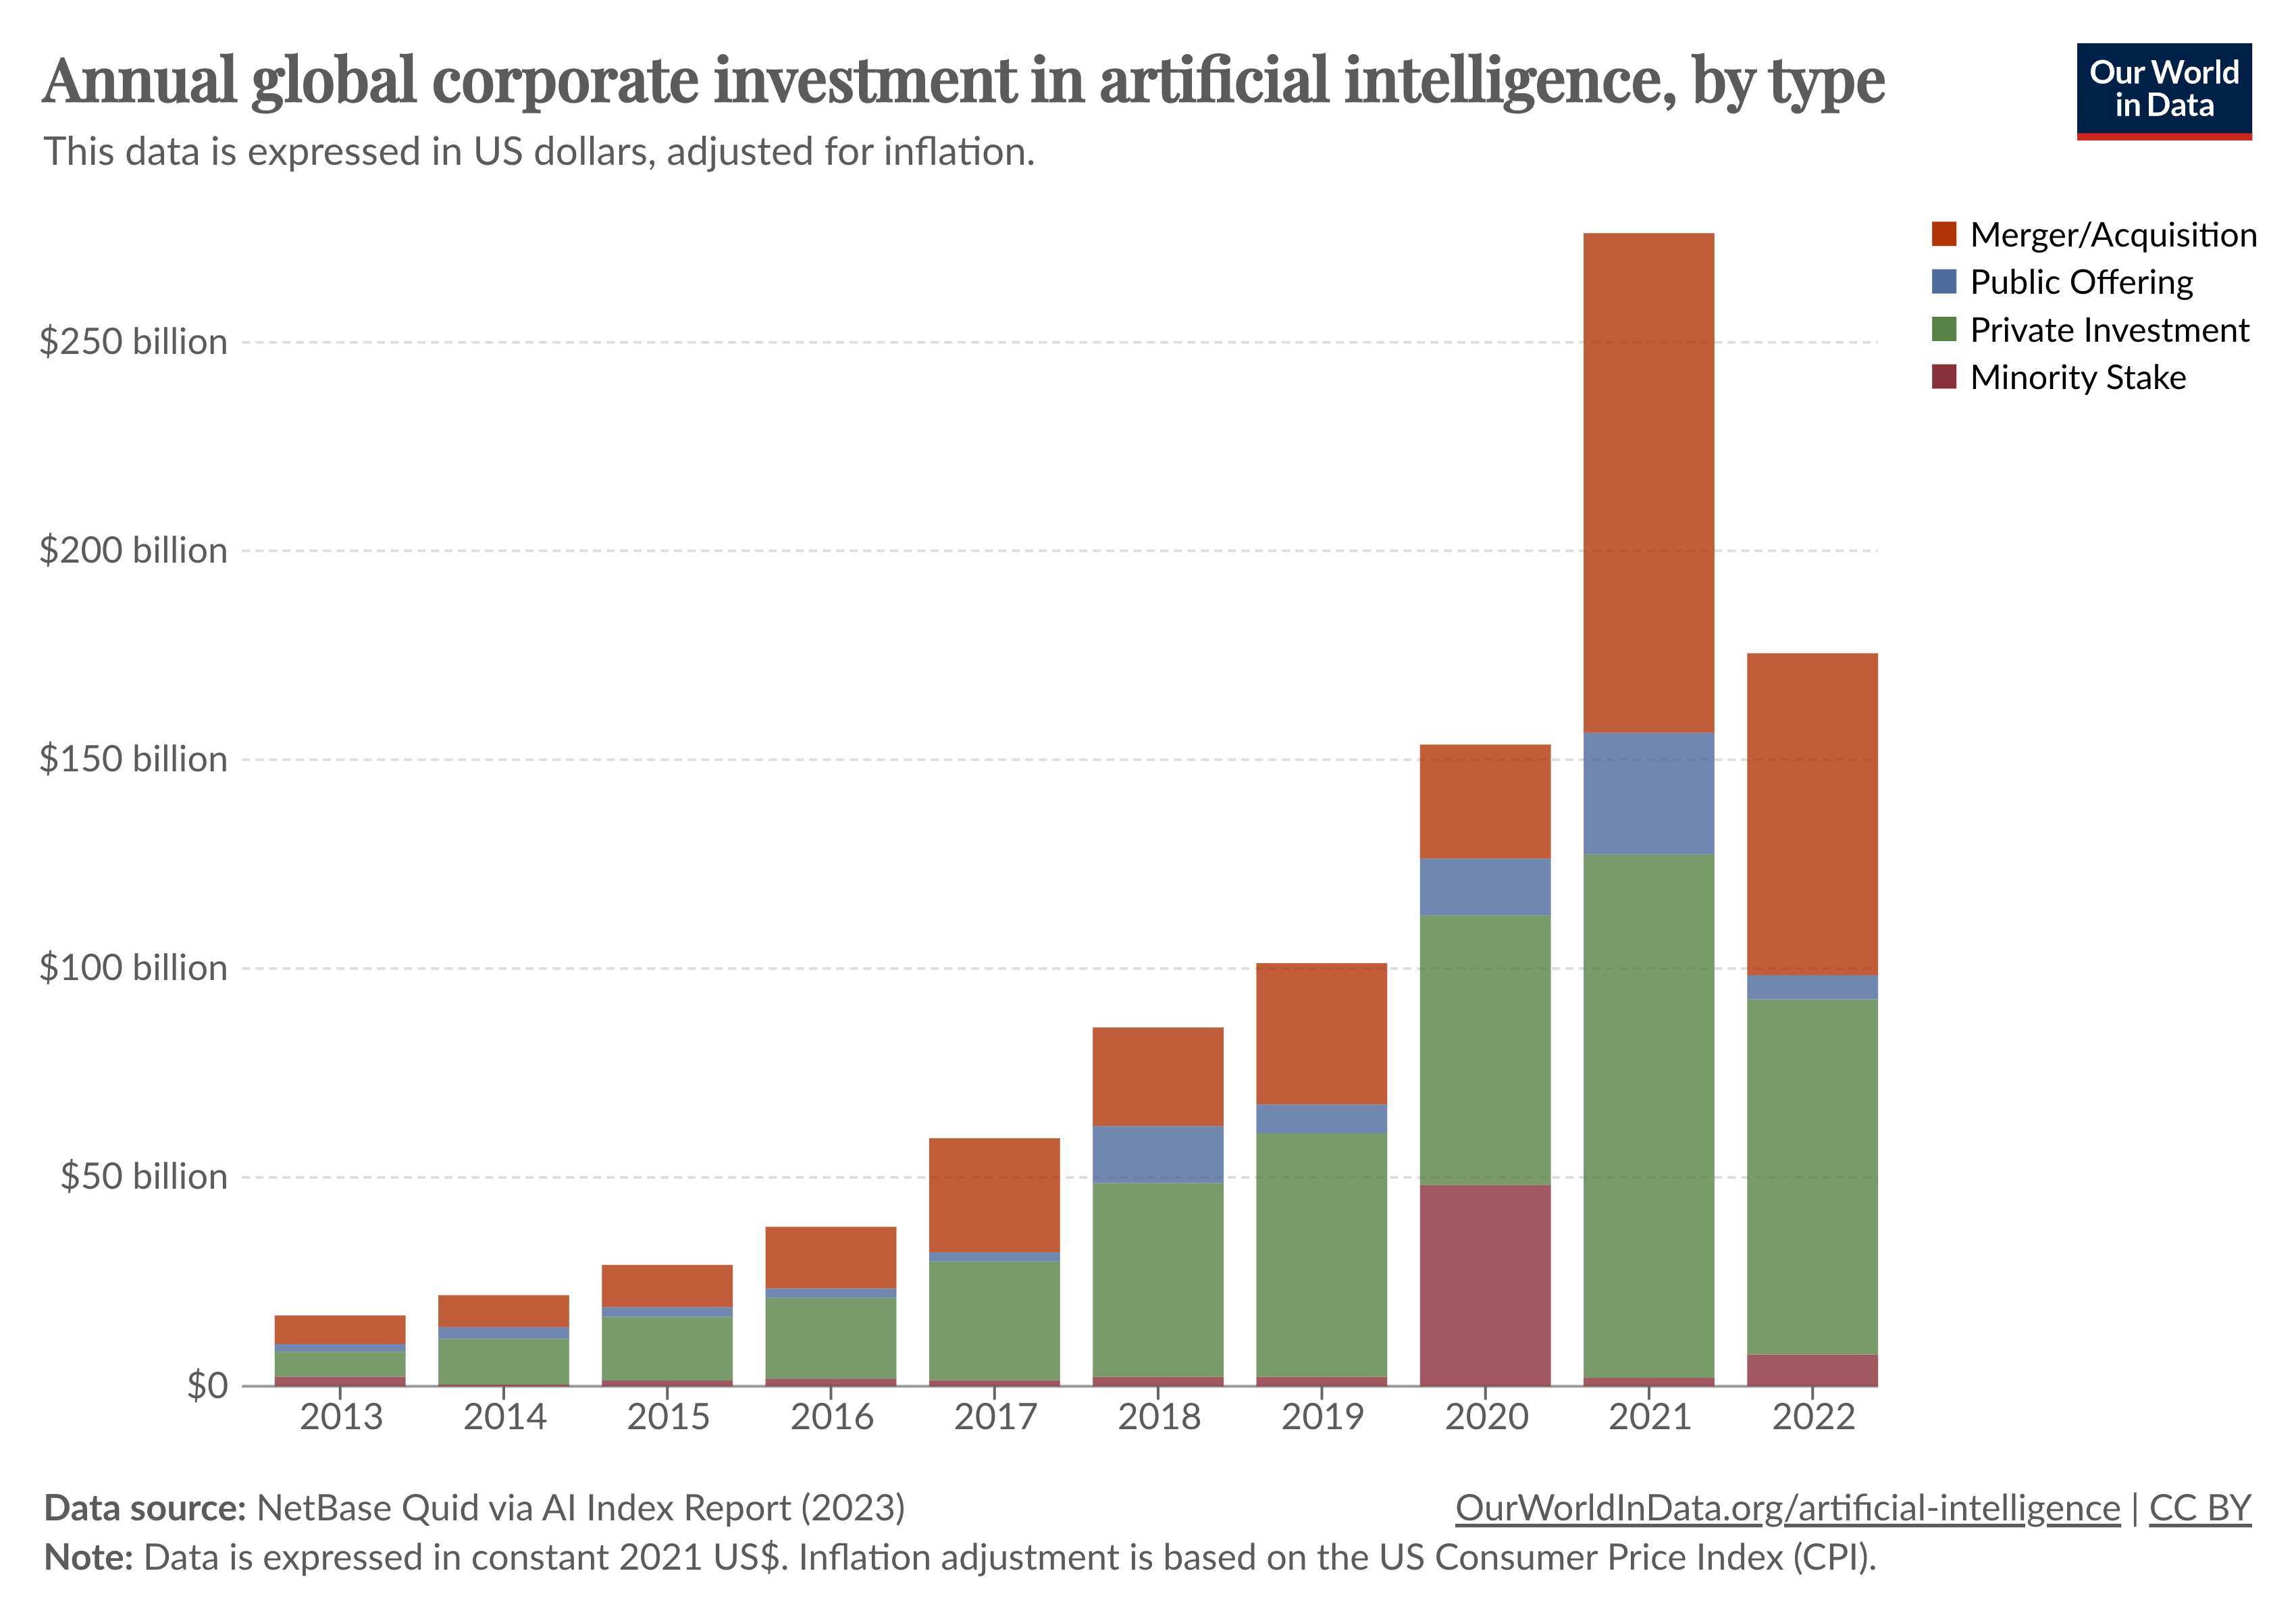
\includegraphics[width=\linewidth]{./data/investment_by_type.png}
        \caption{Annual investment in AI by type}
        \label{fig:investment}
    \end{minipage}\hfill
    \begin{minipage}[t]{0.48\linewidth}
        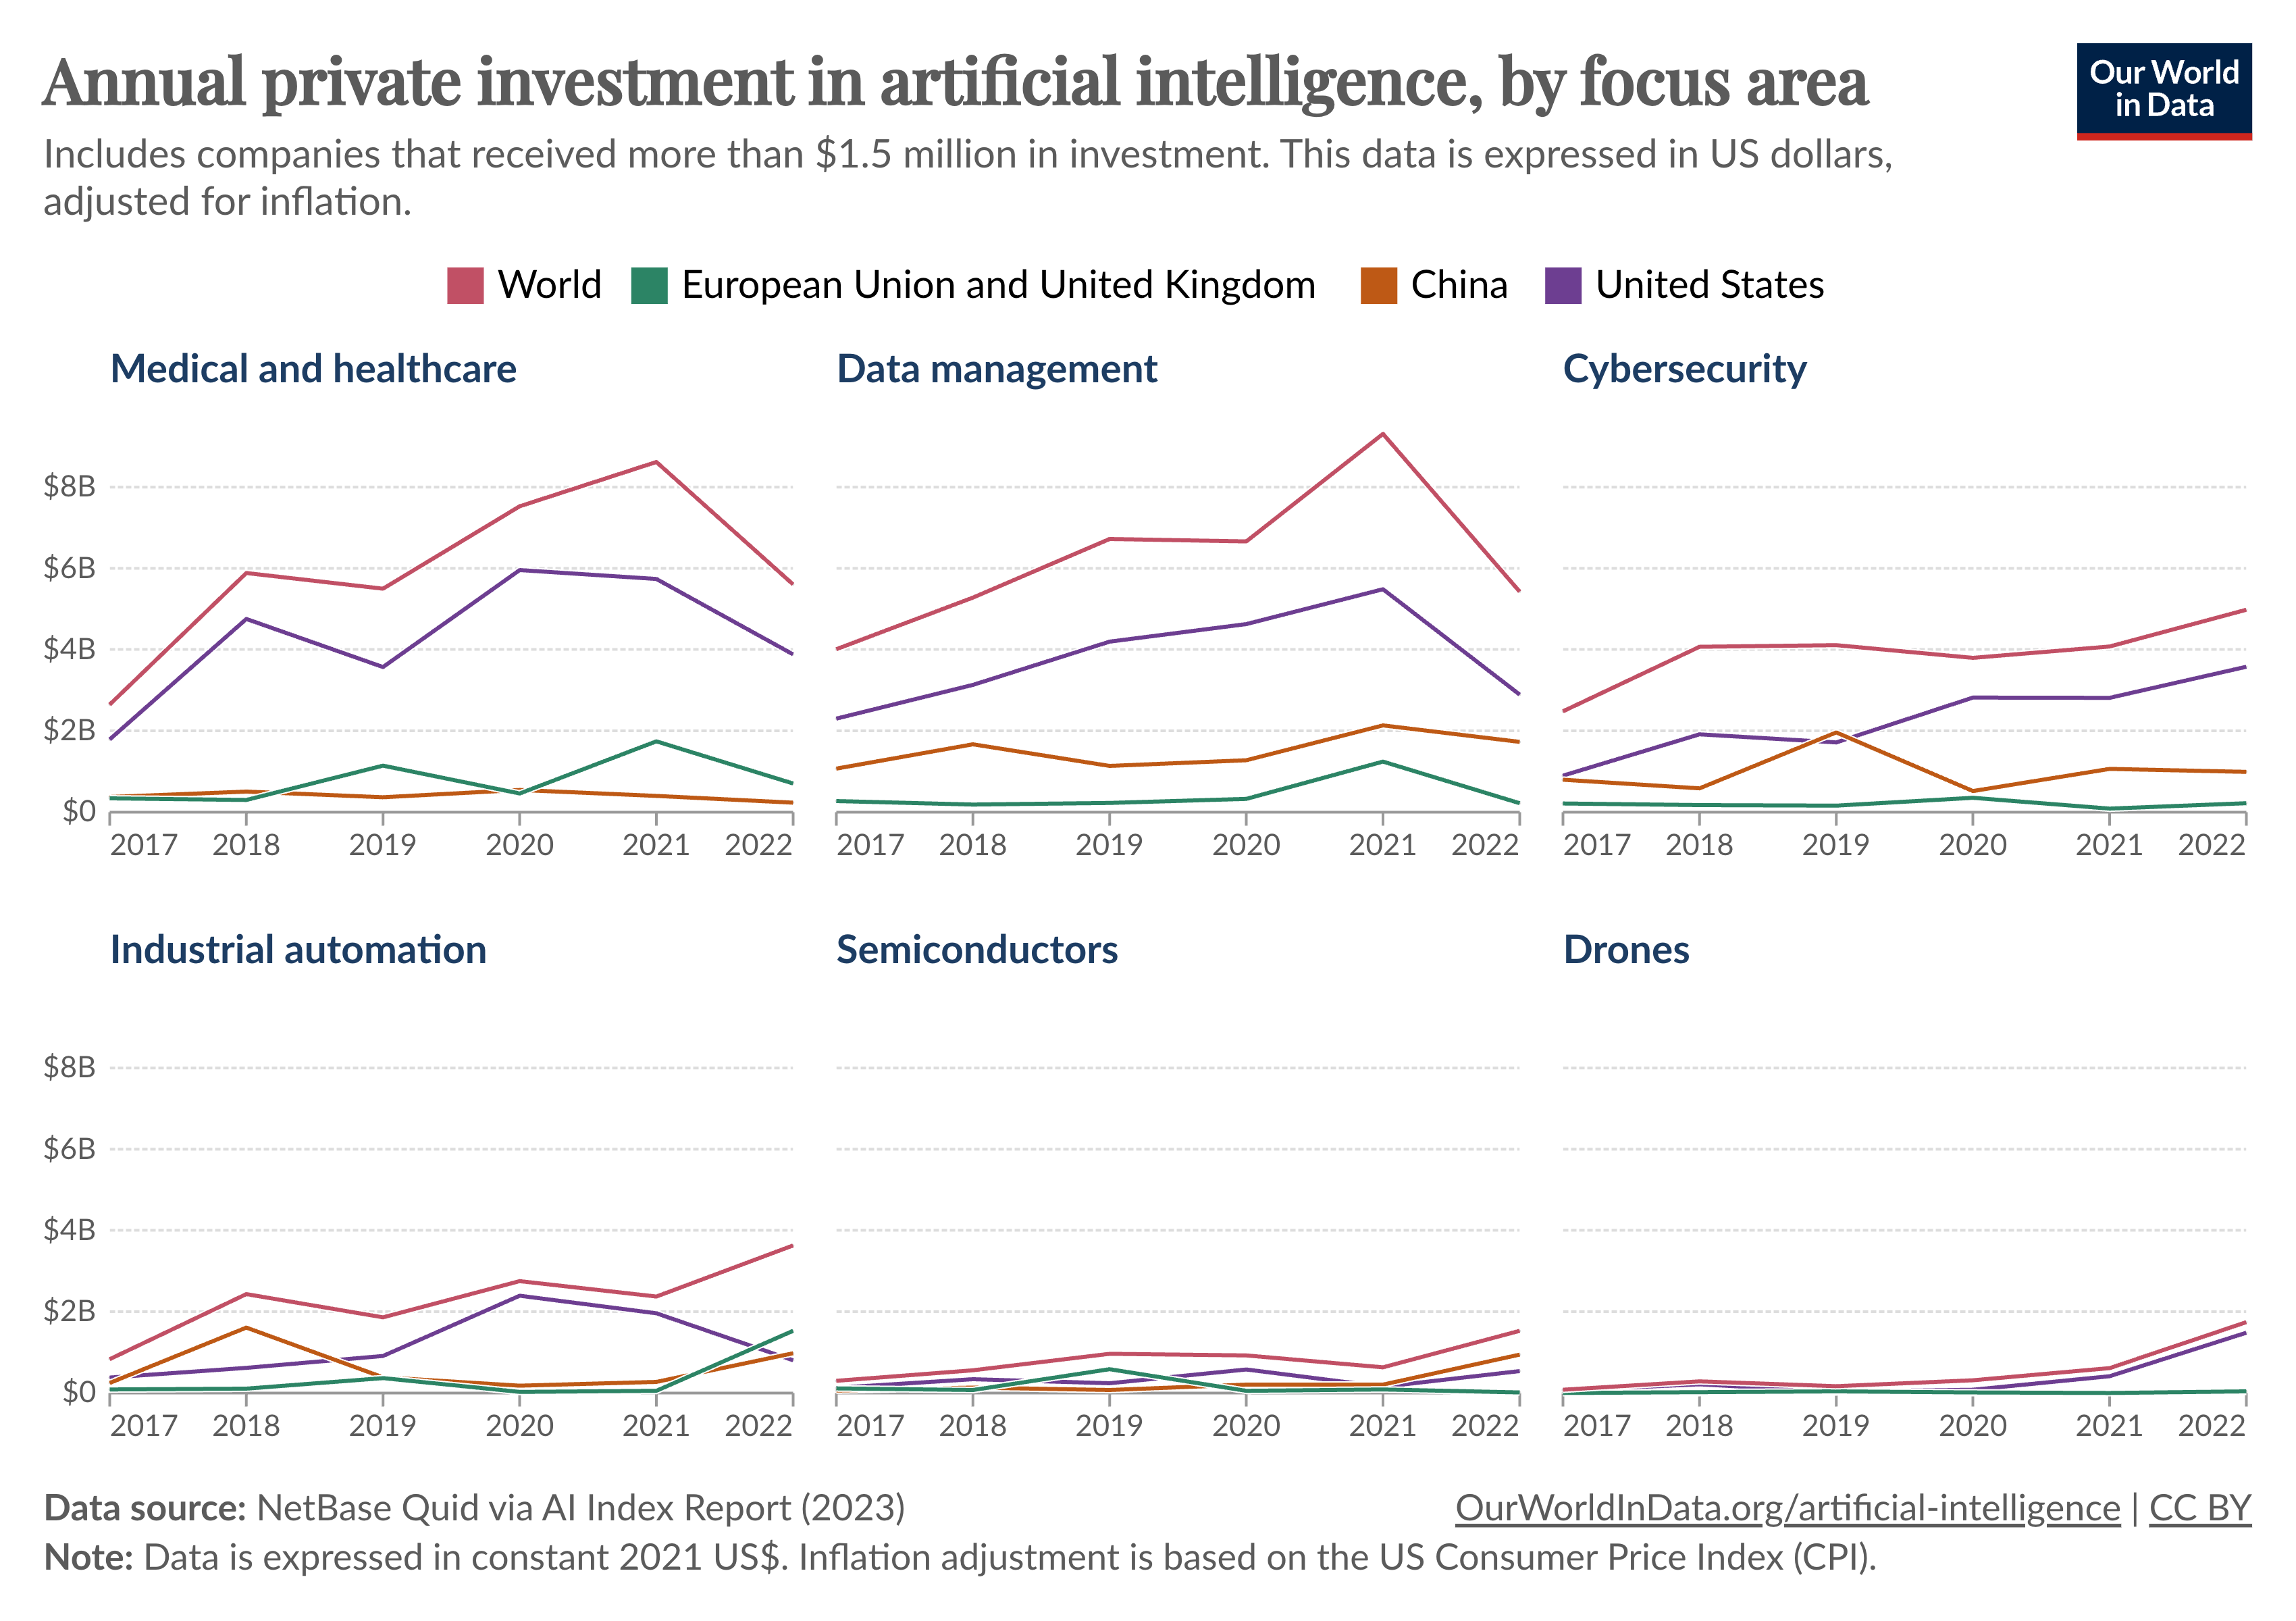
\includegraphics[width=\linewidth]{./data/investment_by_area.png}
        \caption{Annual investment in AI by area}
        \label{fig:views_ai_impact}
    \end{minipage}
\end{figure}


% 隐私和数据保护
\section{Privacy and data protection}
In the realm of Healthcare AI, the protection of patient privacy and data is paramount. 
Patients express concerns about the use of their sensitive information, such as medical 
records and test results, which are stored in hospital databases. They question the duration 
of data storage, access by staff, purposes of data use, and potential for unauthorized sharing \cite{JayasundaraETHICALISSUESSURROUNDING}. 
Although electronic records offer increased security compared to paper files, there remains a 
risk of cyberattacks and internal visibility. The implications of data breaches are profound, 
affecting personal life through potential bullying, increased insurance costs, and job loss 
due to disclosed medical history \cite{Thapa2021PrecisionHealthData}. Therefore, ensuring robust data protection measures and 
transparency in data handling is essential for maintaining trust in healthcare services.


% 信任
\section{Transparency and Trust}
The pervasive "black box" nature of AI algorithms fuels transparency and trust issues 
in Healthcare AI (HCAI). The public's apprehension is amplified by concerns over HCAI's 
recommendations for diagnosing and treating medical conditions, despite physician oversight \cite{esmaeilzadehPatientsPerceptionsHuman2021}. 
This skepticism is particularly strong among older individuals and those with lower economic 
status, who fear AI may bring more harm than good. The lack of direct experience with HCAI 
and a basic understanding of AI contribute to a global sentiment of unease about AI's societal 
impact in the coming decades.

\begin{figure}[H]
    \centering
    \begin{minipage}[t]{0.48\linewidth}
        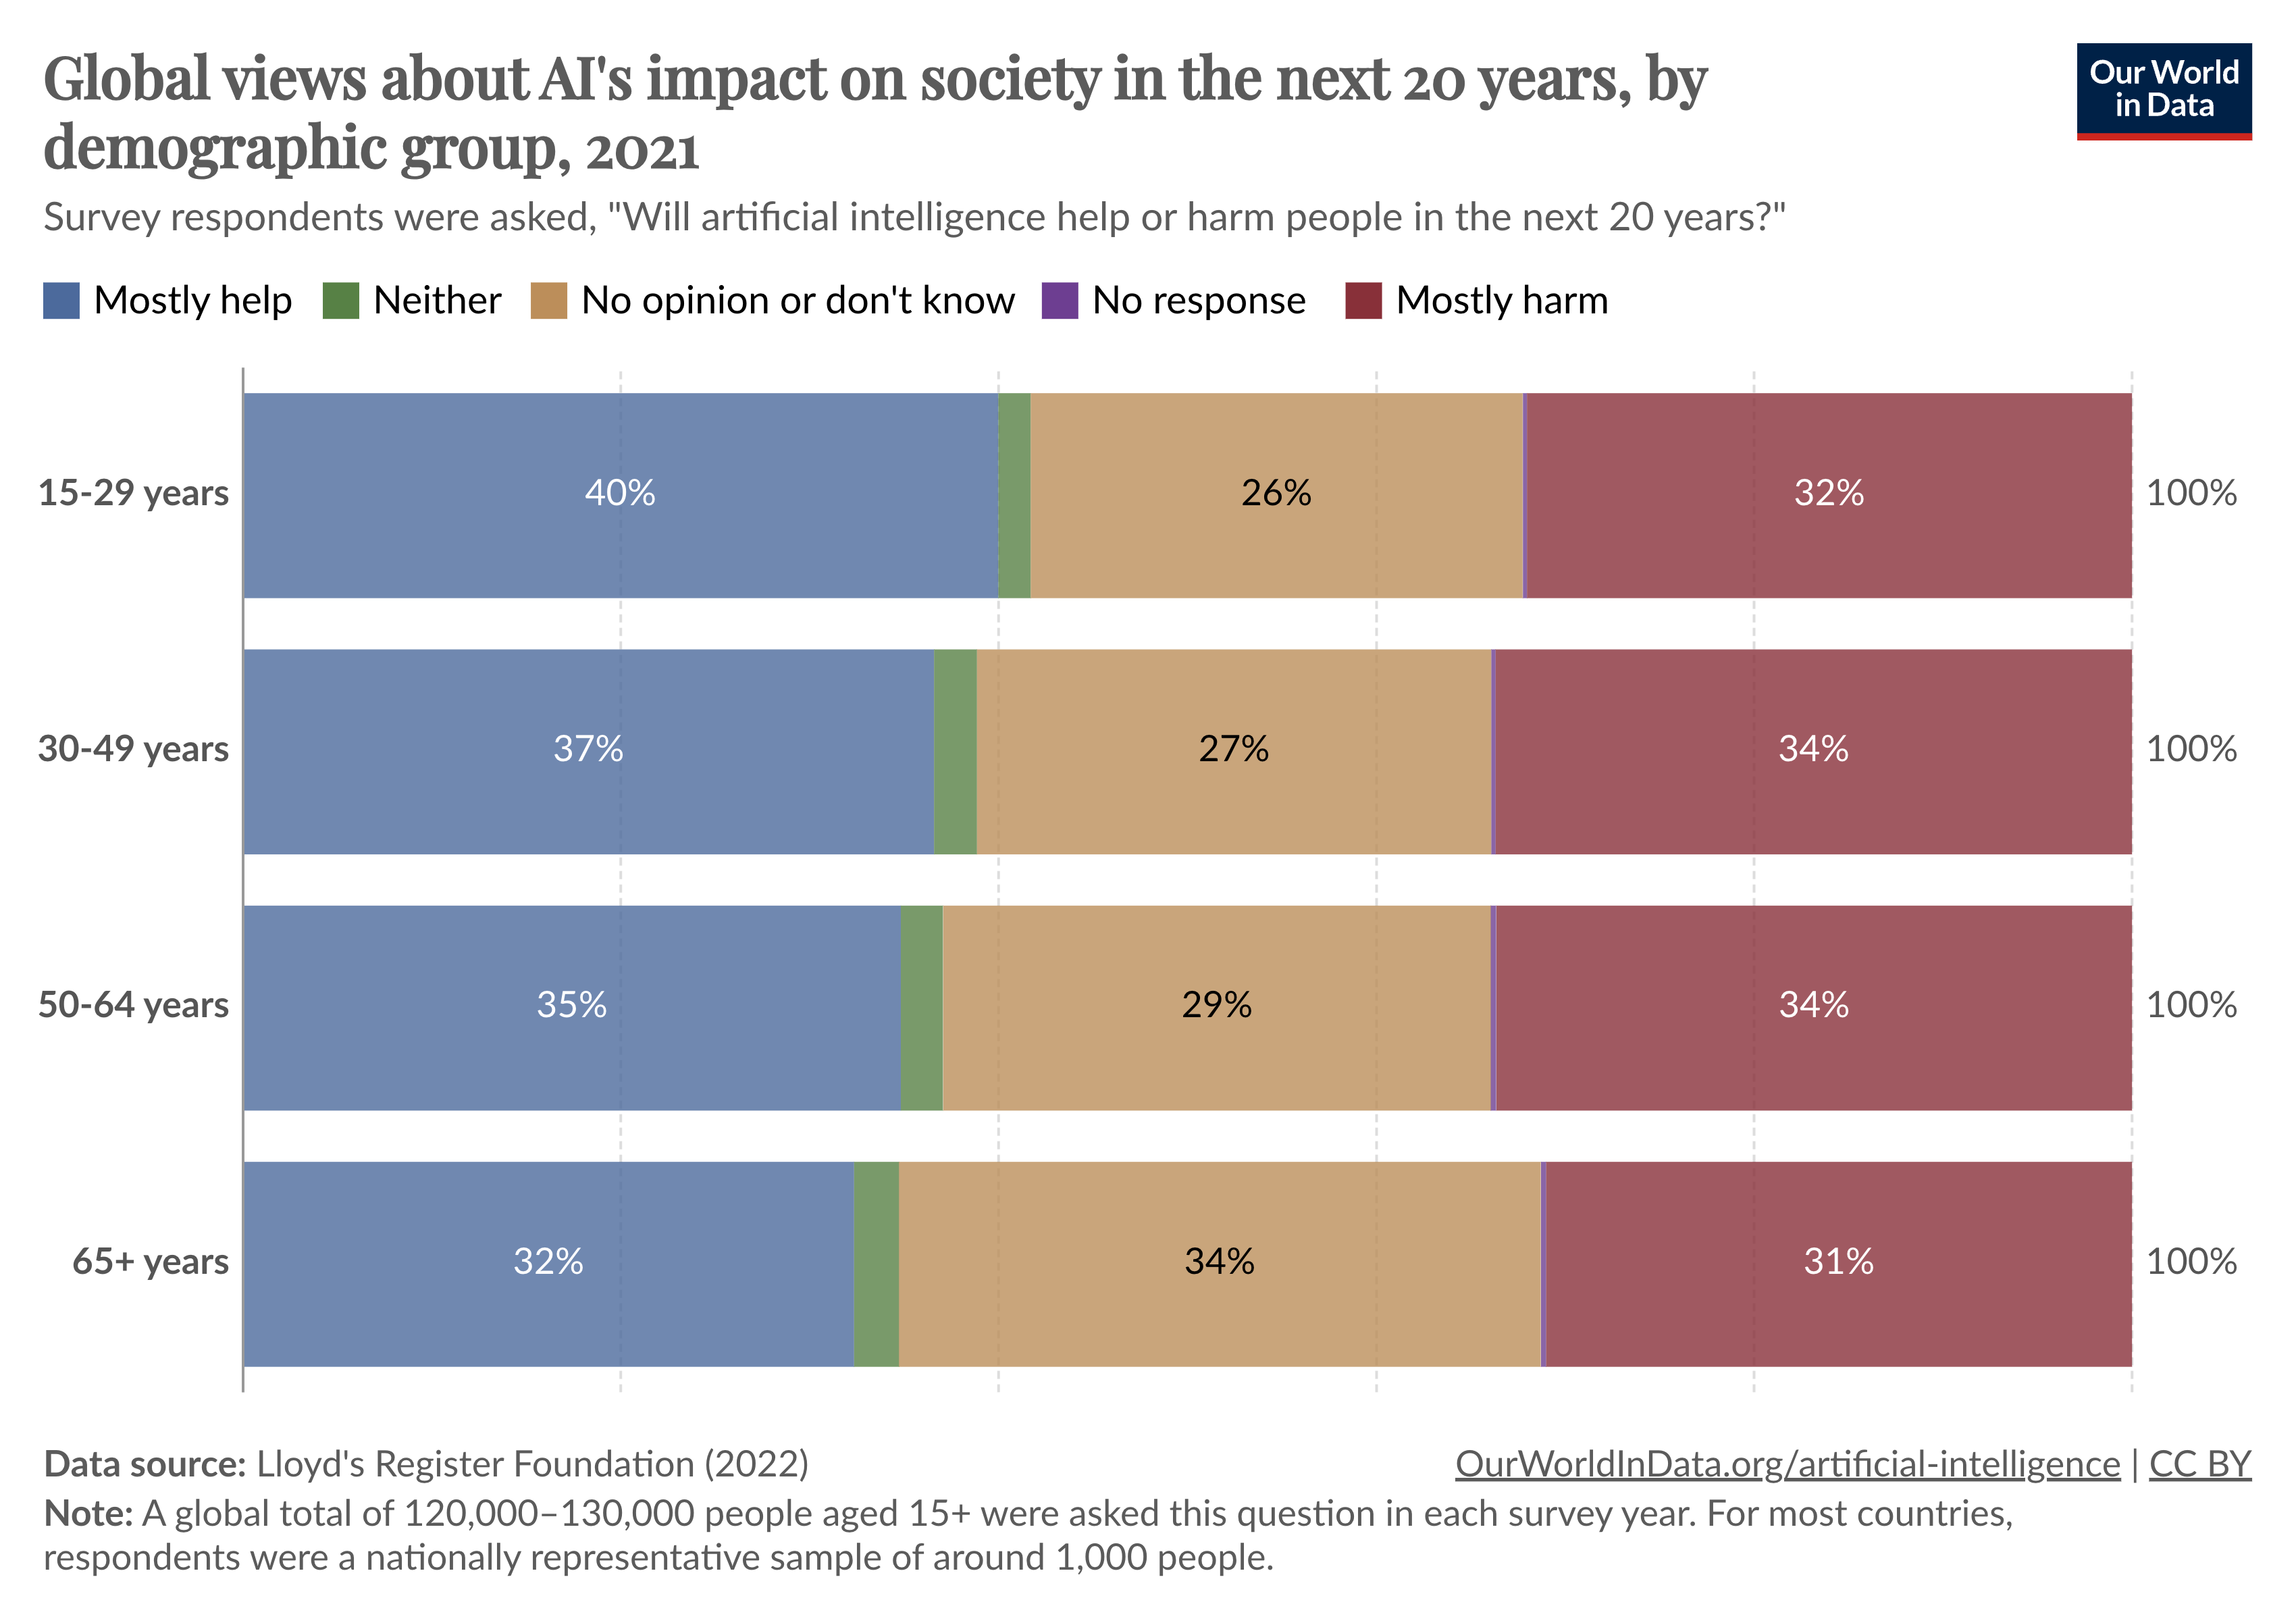
\includegraphics[width=\linewidth]{./data/influence_by_ages.png}
        \caption{Views on AI's impact on society by ages}
        \label{fig:investment}
    \end{minipage}\hfill
    \begin{minipage}[t]{0.48\linewidth}
        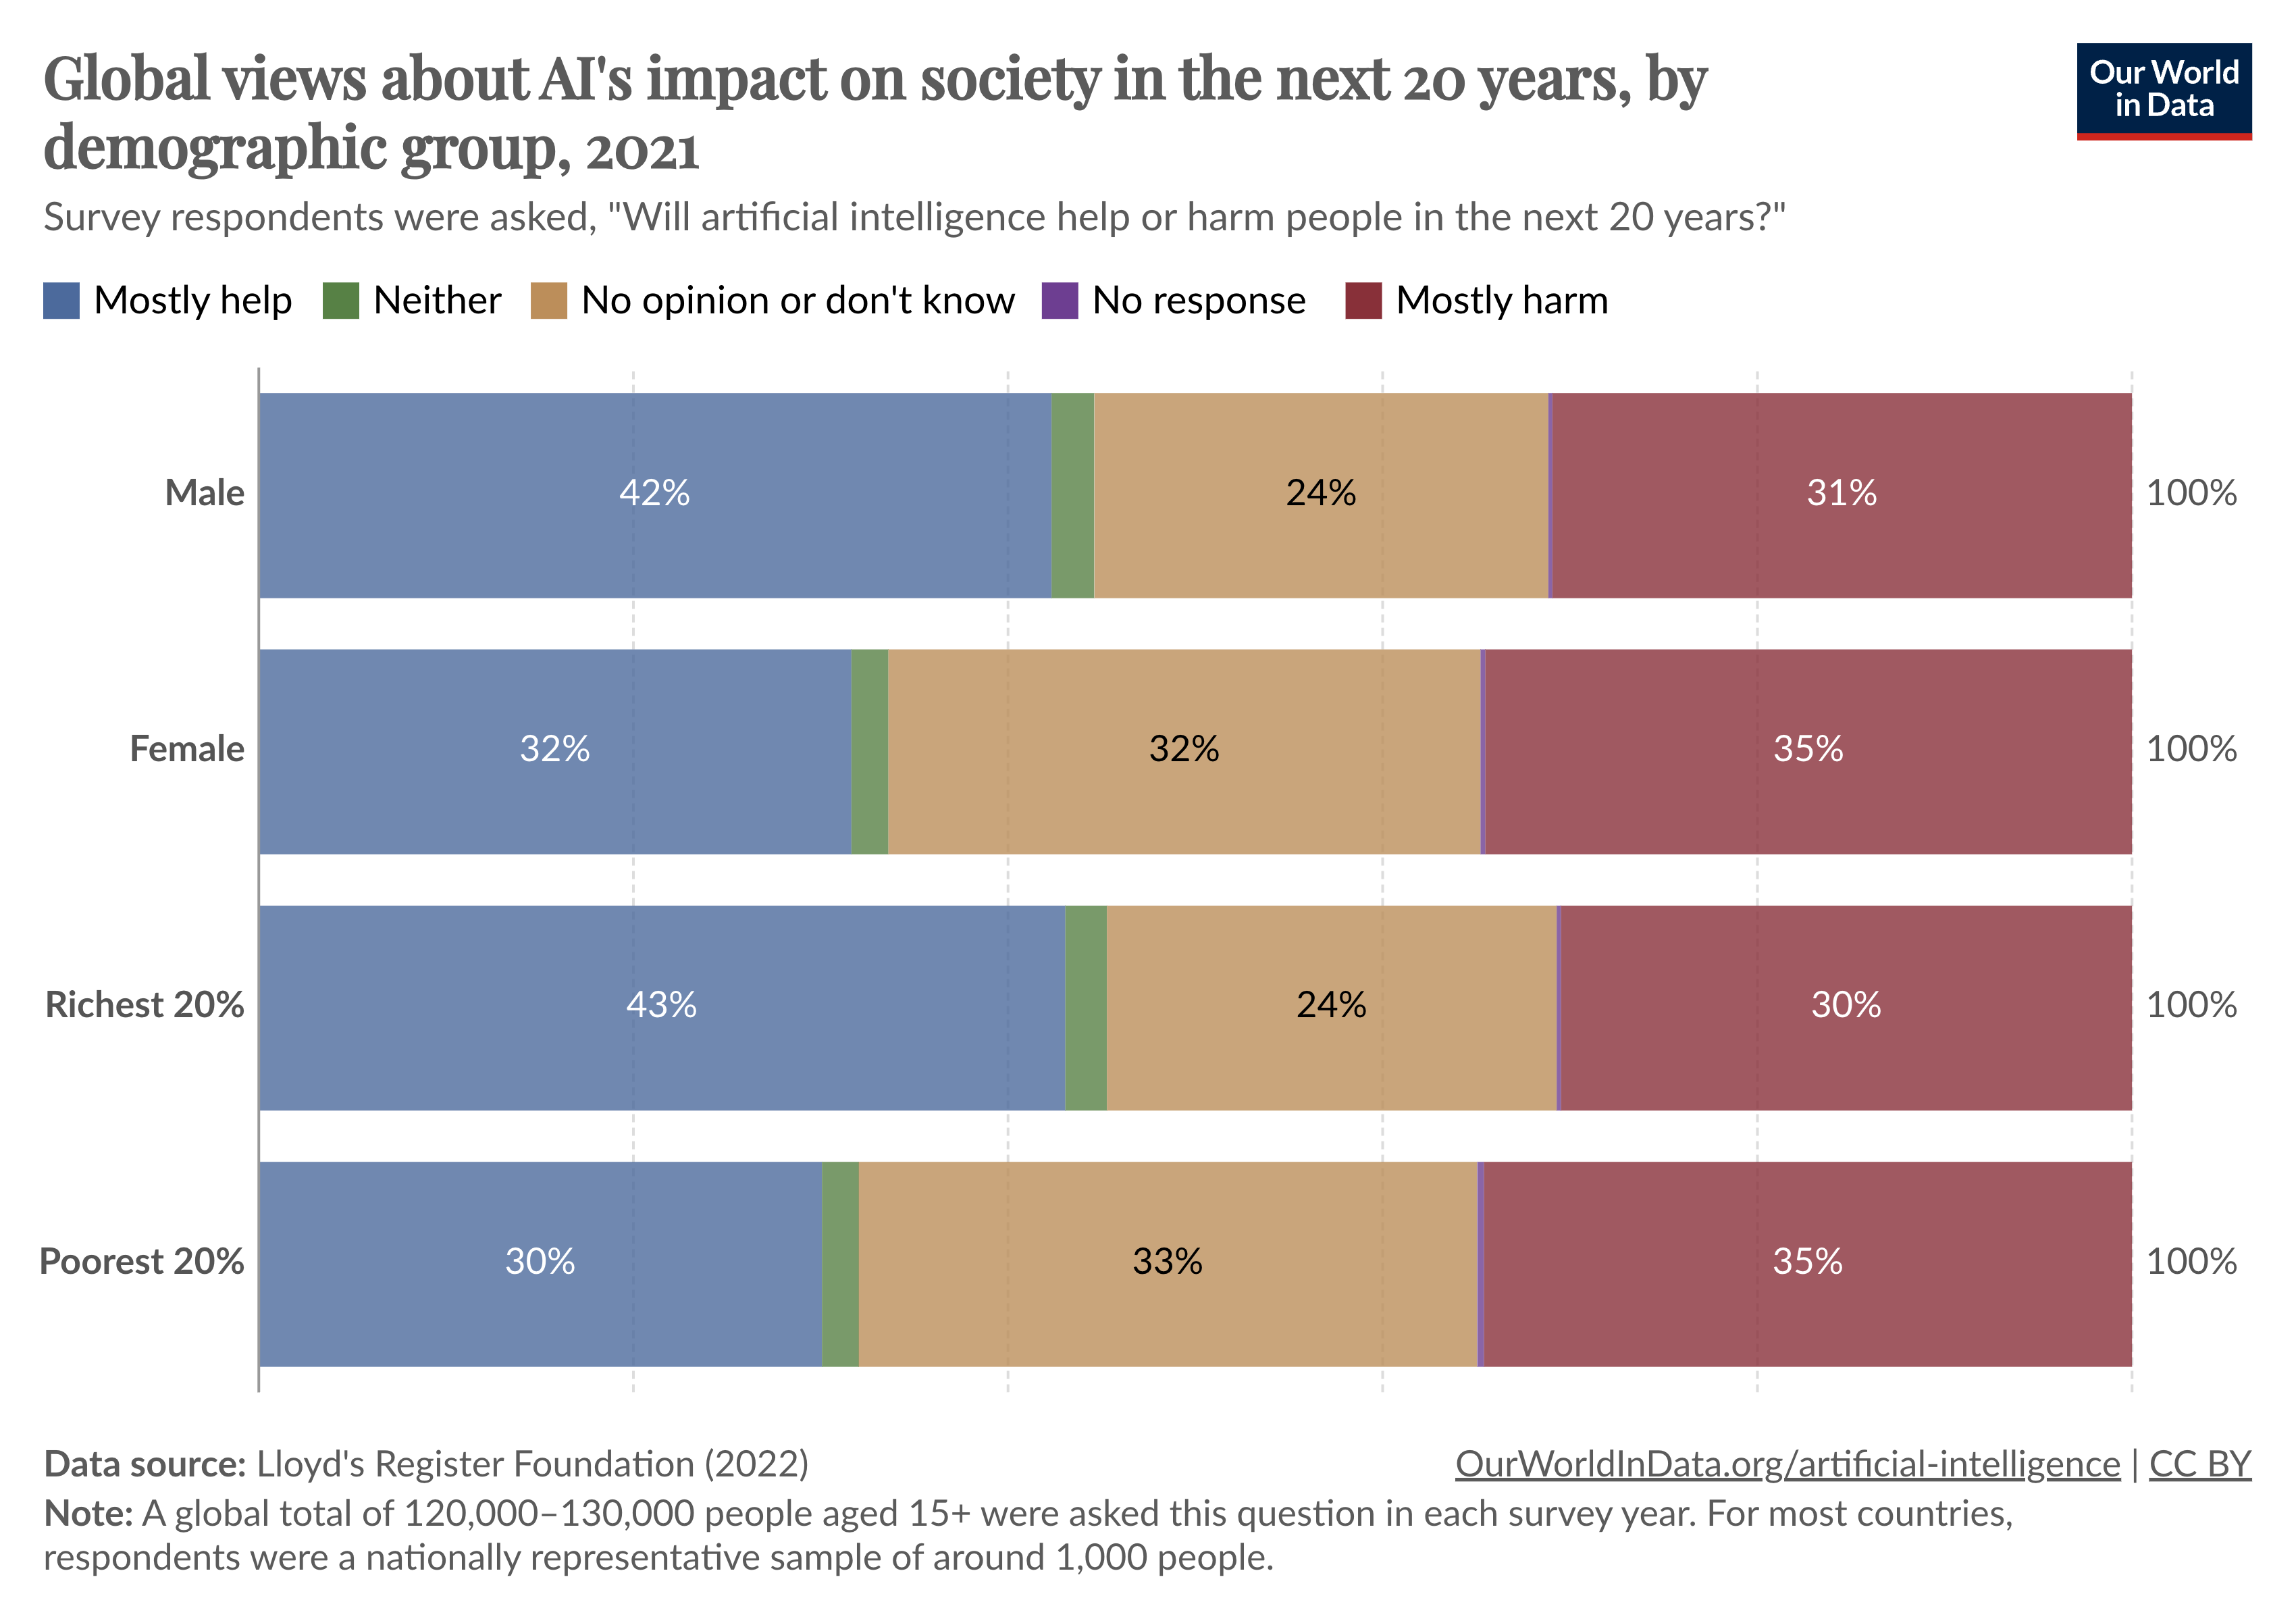
\includegraphics[width=\linewidth]{./data/influence_by_demographic_group.png}
        \caption{Views on AI's impact on society by gender and wealth}
        \label{fig:views_ai_impact}
    \end{minipage}
\end{figure}


% 机器与人类合作
\section{Machines and humans collaborate}
Artificial intelligence is heralded as a breakthrough for complex medical tasks, such as accurately interpreting chest X-rays, 
potentially outperforming humans. However, this innovation stirs fear among doctors about being replaced or marginalized, 
highlighting a lack of trust in AI and its developers, which could hamper AI's development in healthcare. 

In Additionally, a national survey in Turkey, involving 167 emergency medicine specialists, 61.68\% trust 
in anonymity to protect privacy, and 70.66\% believe AI systems are unbiased \cite{ahunPerceptionsConcernsEmergency2023}, 
This result indicated a majority downplay ethical concerns about data storage and reuse.

Further more, the people are not just composed of data, not matter docter or a public they all personhood. 
Machines have no personhood and will only give cold conclusions. Medical staff need to maintain professionalism 
and compassion during diagnosis and treatment. If these are lost, it is possible to intensify the mechanization 
and dehumanization of patients, and the unique situation of the patient will be Without being heard.



\section{suggestings}
(1) By educating the public and medical staff on artificial intelligence and related ethical issues, 
this will help to improve their awareness of privacy and human rights in artificial intelligence.
\\(2) By openly acknowledging the value of medical staff and respecting the decisions of clinicians, 
they realize that artificial intelligence is not a competitive relationship but a cooperative relationship, 
and the output of artificial intelligence is communicated to patients in a way that doctors can understand.
\\(3) Implement stringent oversight mechanisms and regulations to ensure HCAI systems are used under 
the guidance of experienced physicians, safeguarding against misdiagnosis or inappropriate treatment suggestions.
\\(4) Based on PCC and EBM care approaches, involve patients in the development and evaluation of HCAI systems to ensure that these technologies 
meet their needs and address their concerns, particularly regarding the mechanization and dehumanization of care \cite{iniestaHumanRoleGuarantee2023}.

\section{Conclusion}


Human fear comes from the unknown, Puclic's anxiety towards HCAI in healthcare stems from a lack of understanding.
Medical staff's anxiety come from the disruption of traditional work models by HCAI. The confusion and panic caused 
in this situation are the fundamental reasons for the moral and ethical problems of artificial intelligence.

Breaking the unknown path is to spread knowledge. When people reveal the mystery of artificial intelligence, the fear hidden in their hearts will be banished.
The path to expel chaos lies in establishing order. When we integrate clear norms and guidance into medical practice, confusion about the future can find direction.


The birth of new things is based on the destruction of existing things. The destruction of the traditional medical system by artificial intelligence is an inevitable 
result of its development. Human panic is also a normal emotional expression. Only by facing it squarely can we solve it.




% \begin{figure}[h]
%     \centering
%     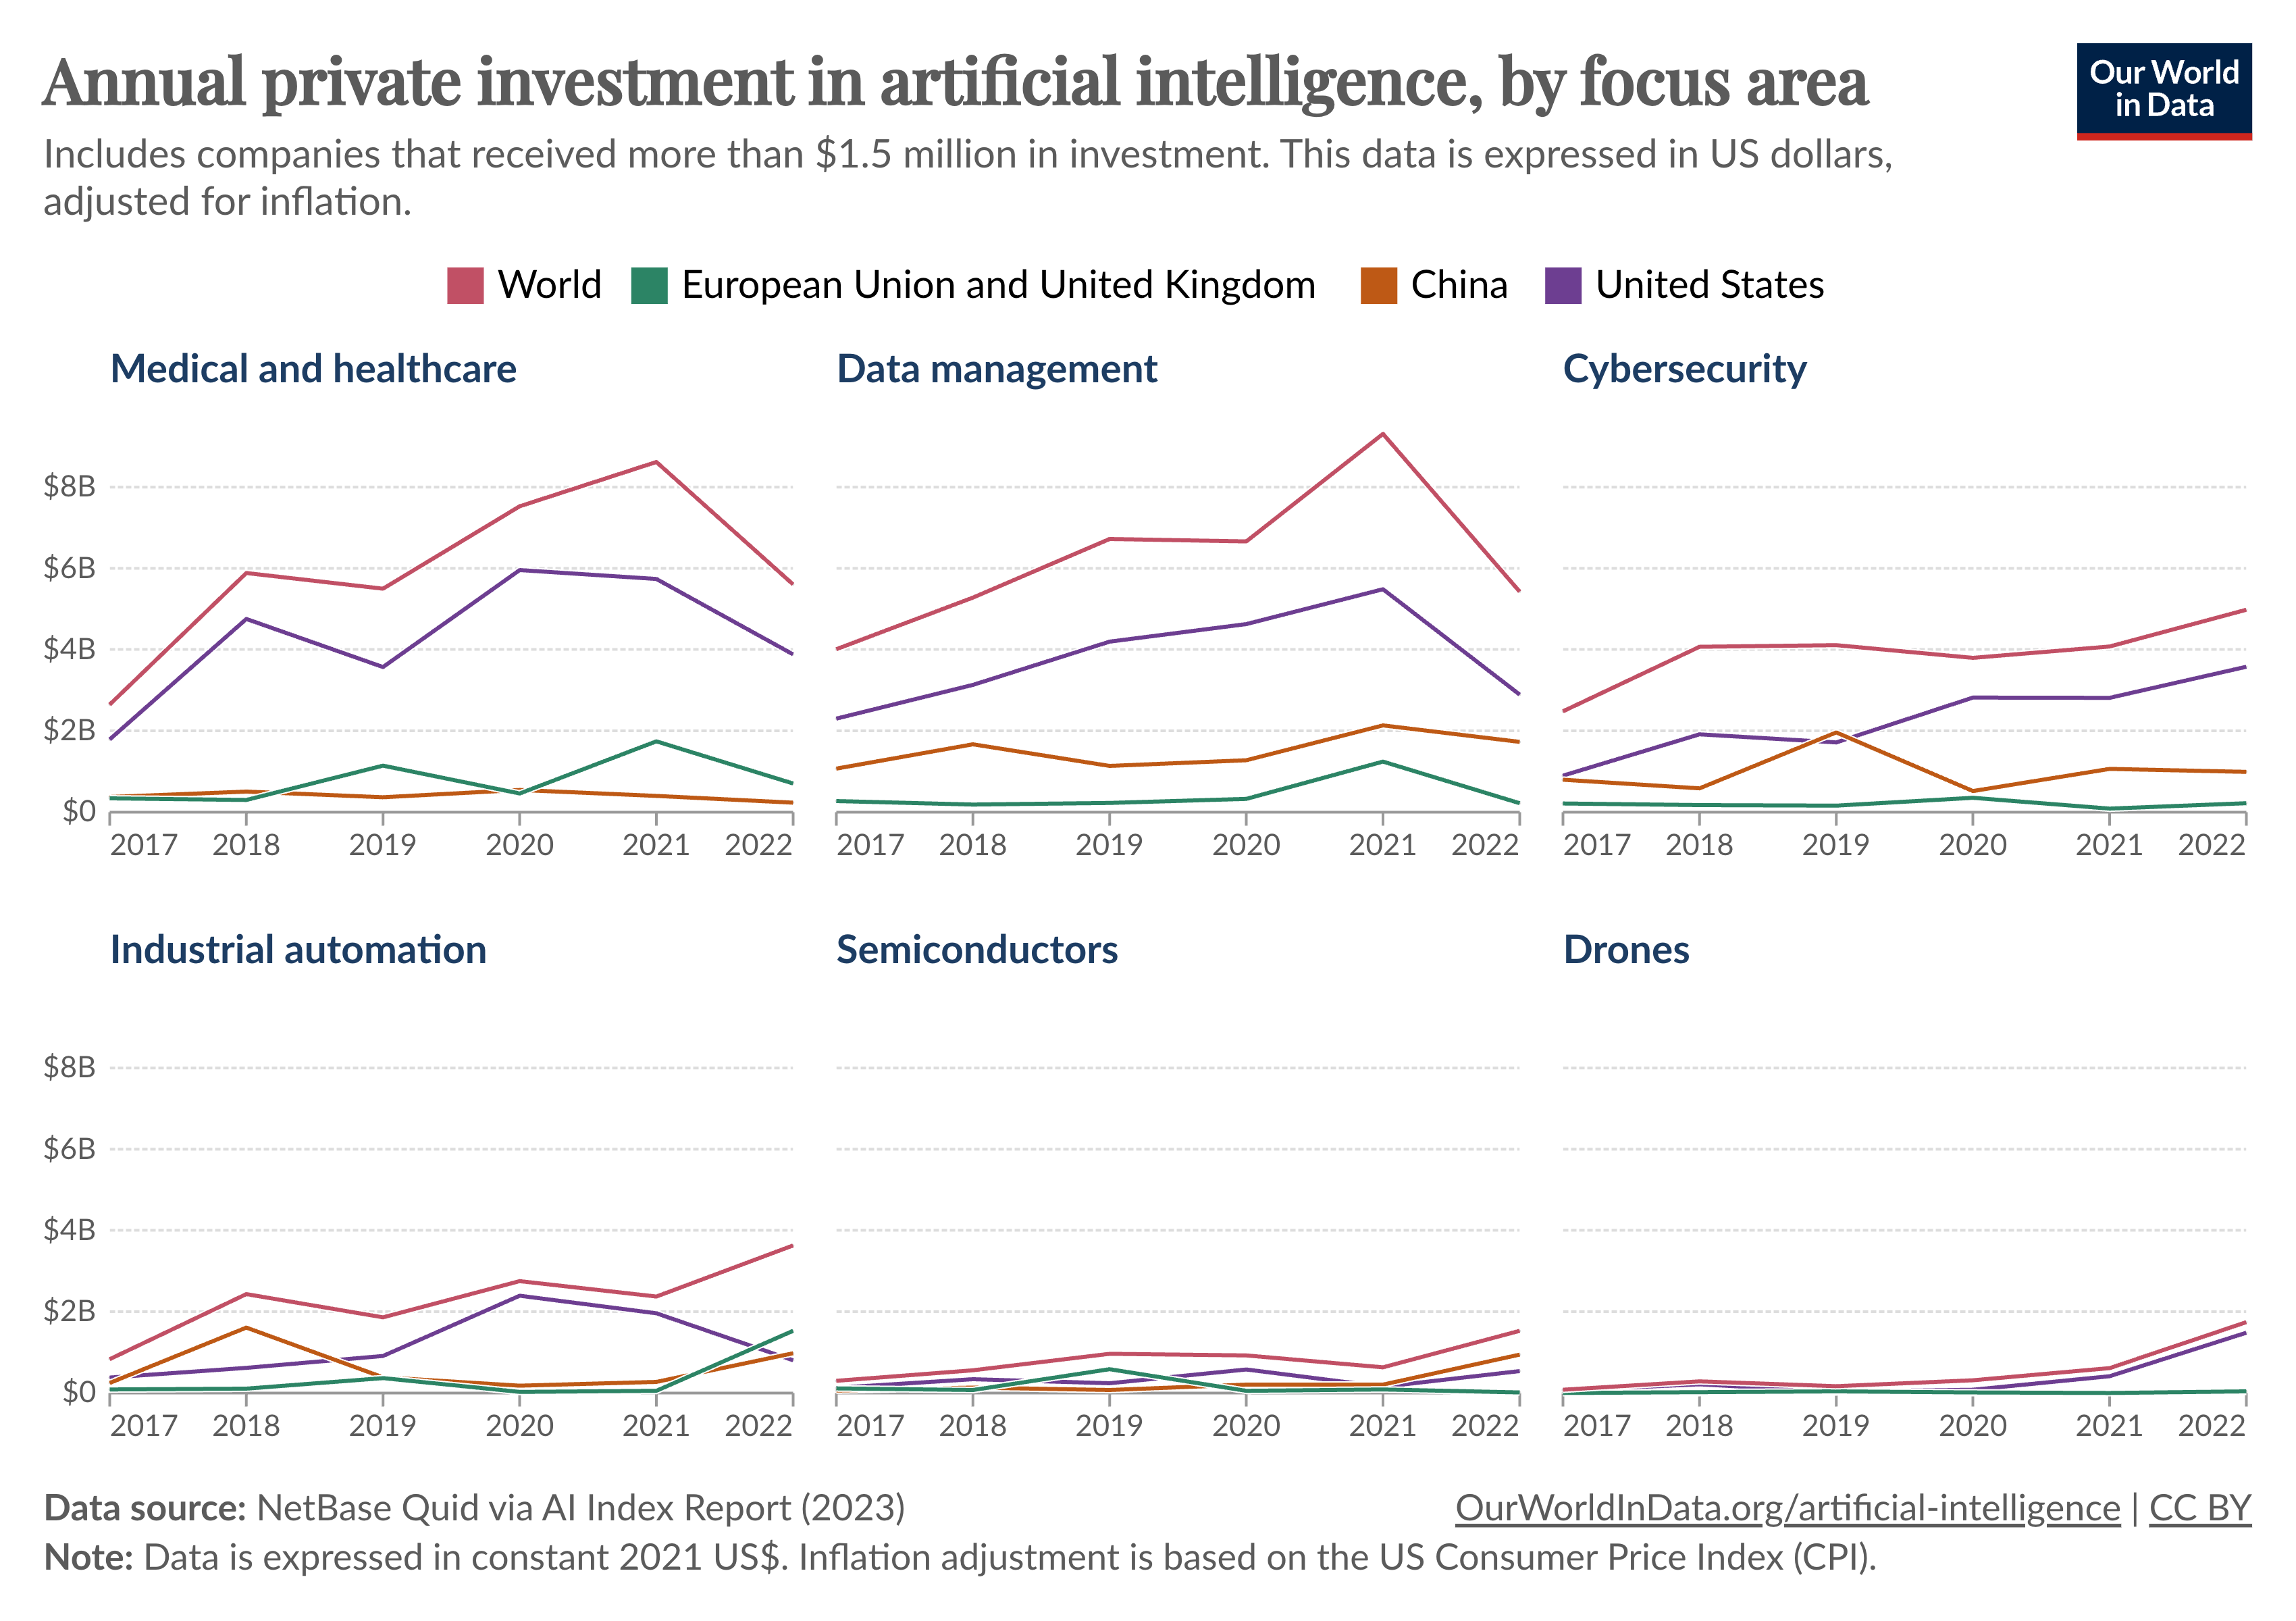
\includegraphics[width=0.9\textwidth]{./data/investegatement.png}
%     \caption{This is the title}
%     \label{fig:my_picture}
% \end{figure}



% \begin{figure}[h]
%     \centering
%     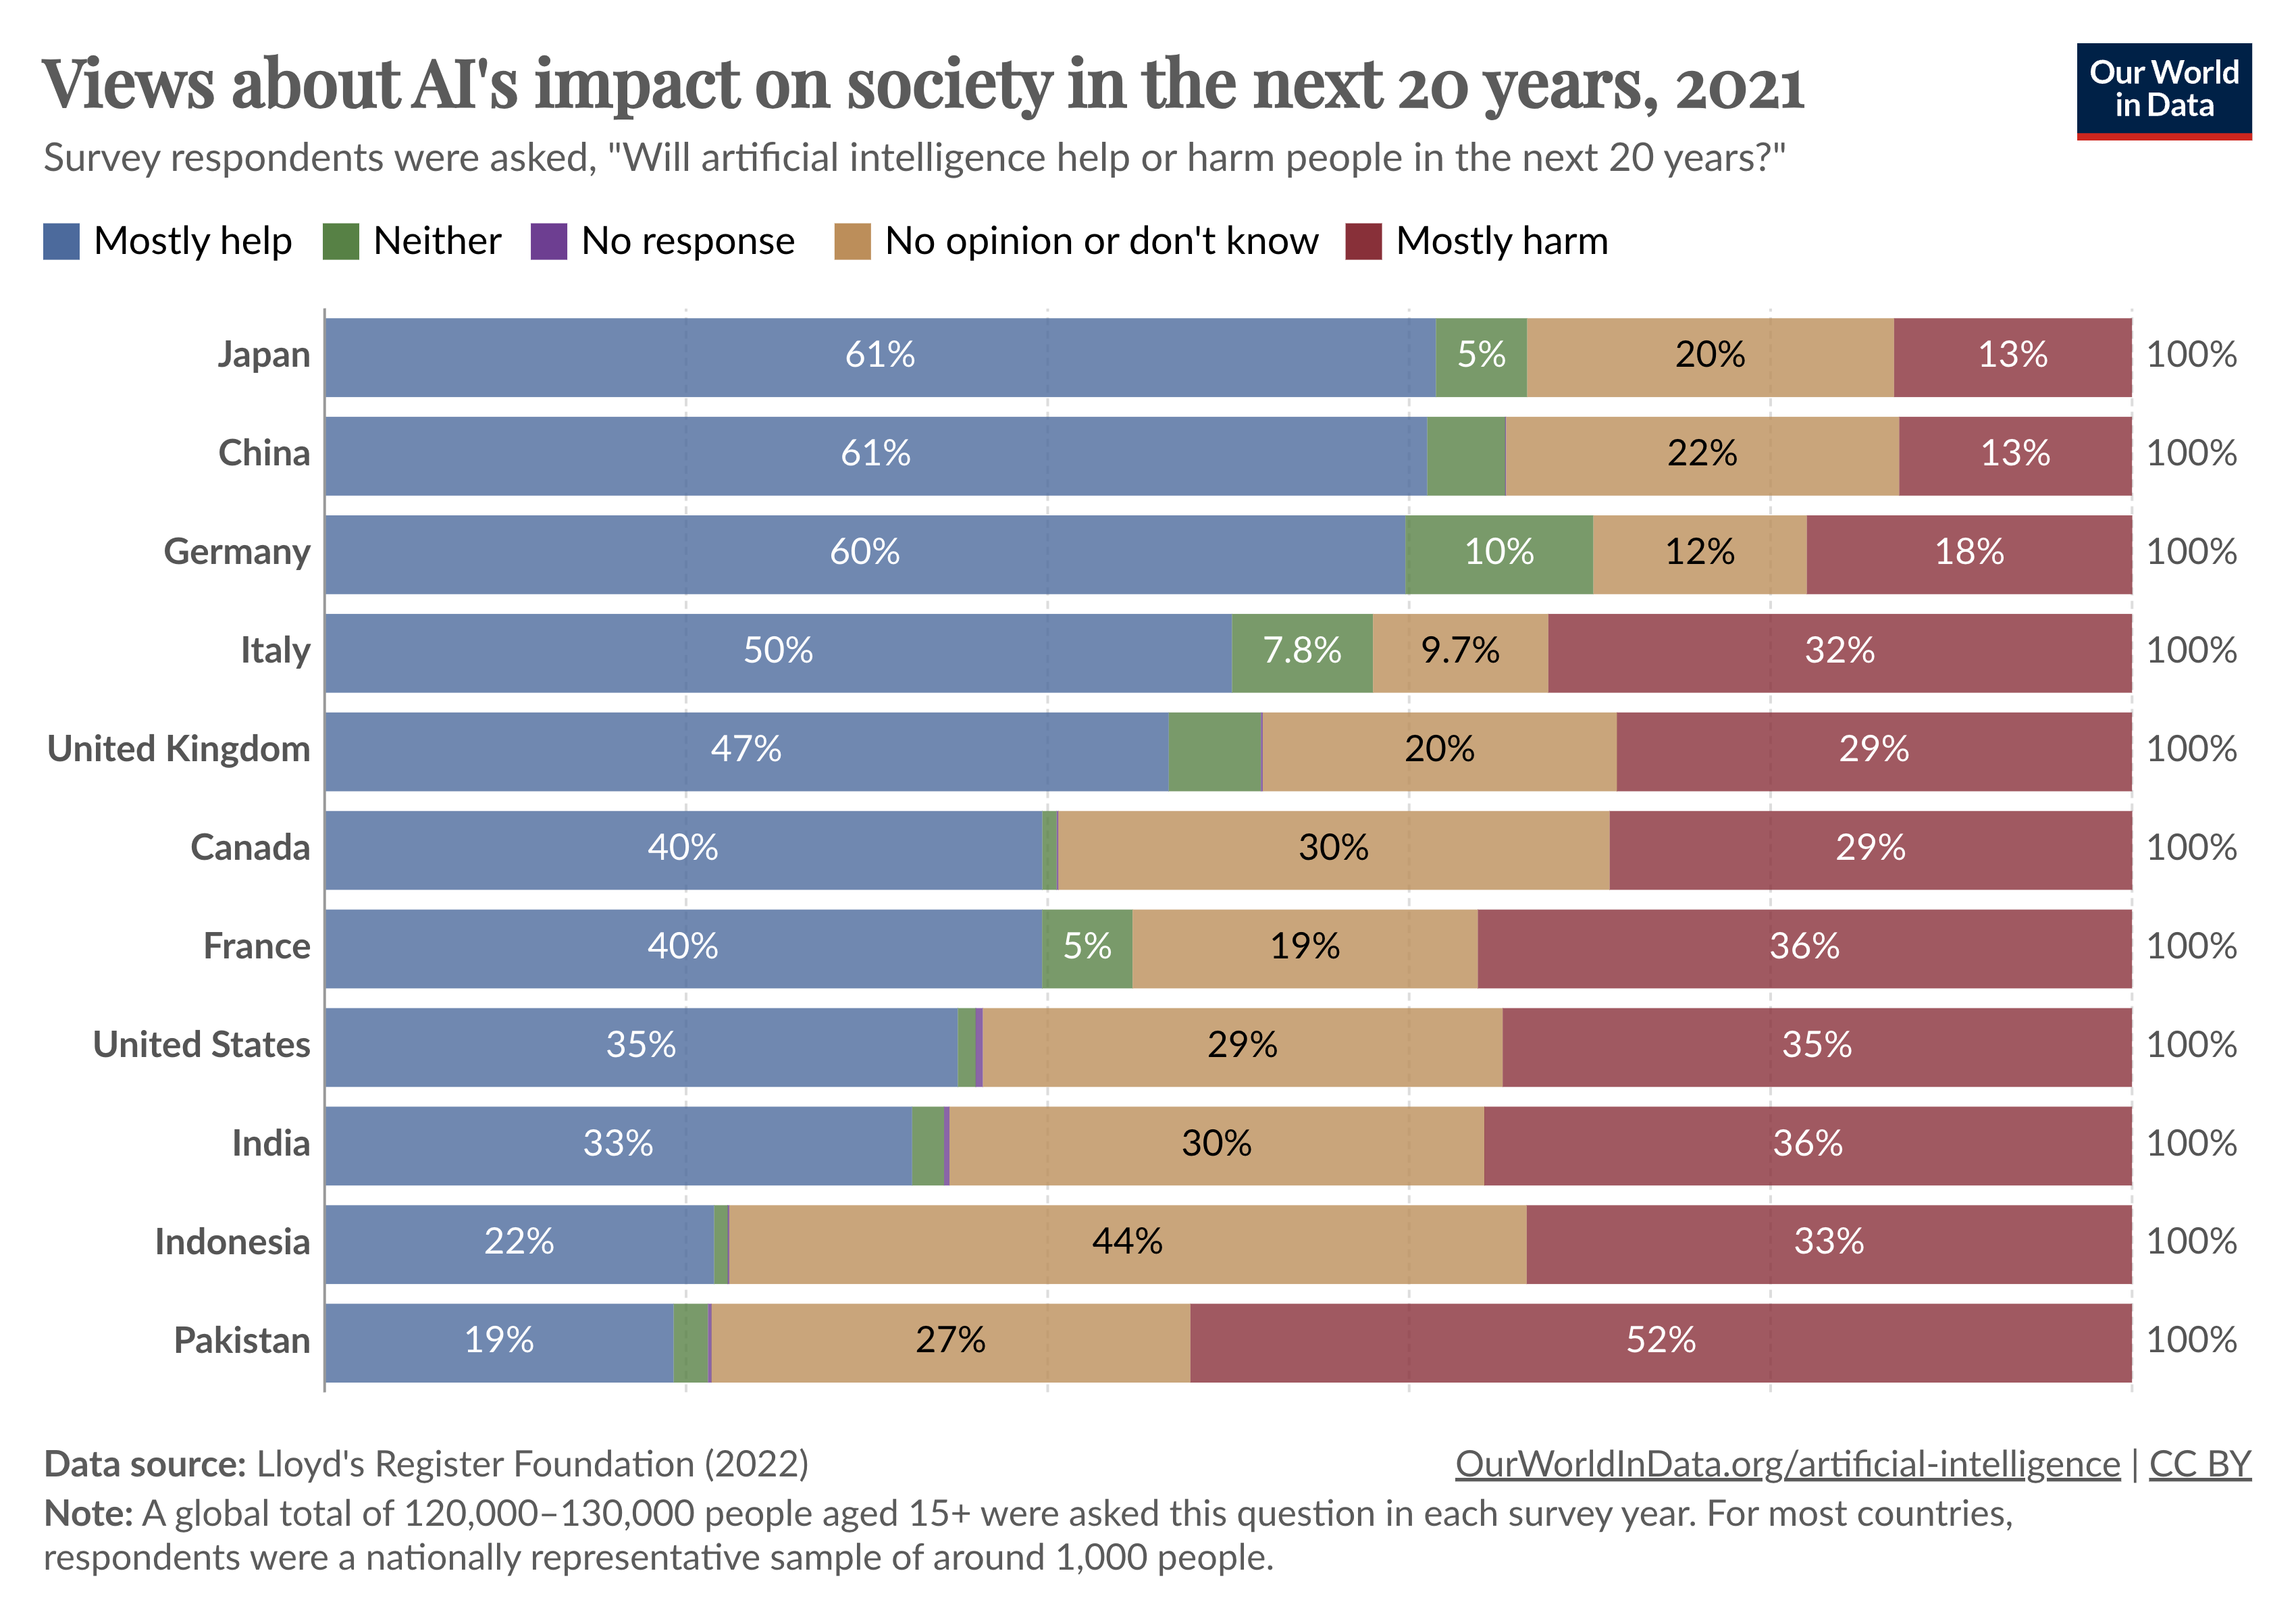
\includegraphics[width=0.9\textwidth]{./data/influence.png}
%     \caption{This is the title}
%     \label{fig:my_picture}
% \end{figure}
















%----------------------------------------------------------------------------------------

\bibliographystyle{unsrt} % This specifies the style of the bibliography
\bibliography{/Users/dengkai/workspace/papers/latex/config/ref} % This should match the name of your .bib file without the extension
\end{document}

